\subsection{Fórmulas explícitas para los primeros vectores (máximo hasta el cuarto) de la base $\cali{L}^{n}$}

Sea $n \geq 2$.
\begin{itemize}
\item Para toda $0 \leq m \leq n-1$, 

\begin{equation}
\label{eq: Ln, 0, m}
\cali{L}^{n,0}_{m}=\frac{1}{\sqrt{n}}.
\end{equation}

\item \textbf{Fórmula para los polinomios de legendre discretos
de grado $k=1$}
\[
\cali{L}^{n,1}_{m}=\sqrt{\frac{3(n-1)}{n(n+1)}} \left( \frac{2}{n-1}m -1. \right),
\]
o sea, 
\begin{equation}
\label{eq: Ln, 1, m}
\cali{L}^{n,1}_{m}=\frac{2\sqrt{3}}{(n+1)n(n-1)} \left( m-\frac{n-1}{2} \right)
\end{equation}

\item \textbf{Fórmula para los polinomios de legendre discretos
de grado $k=2$} si $n \geq 3$,
\[
\cali{L}^{n,2}_{m}=\sqrt{\frac{5(n-1)(n-2)}{n(n+1)(n+2)}} \left(1- \frac{6}{n-1}m + \frac{6}{(n-1)(n-2)}m(m-1) \right),
\]
o sea, 
\[
\cali{L}^{n,2}_{m}=\frac{6\sqrt{5}}{\sqrt{(n+2)(n+1)n(n-1)(n-2)}} \left(
\left( m-\frac{n-1}{2} \right)^{2}+\frac{n-1}{4}(23n-47)
\right)
\]


\item \textbf{Fórmula para los polinomios de legendre discretos
de grado $k=3$} si $n \geq 4$,
\[
\cali{L}^{n,3}_{m}=-\sqrt{\frac{7(n-1)(n-2)(n-3)}{(n+3)(n+2)(n+1)n}}
\left( 1- A_{n}m + B_{n}m(m-1)-
C_{n}m(m-1)(m-2) \right),
\]
donde
\[
A_{n}:= \frac{12}{n-1},
\]
\[
B_{n} := \frac{30}{(n-1)(n-2)}
\]
y
\[
C_{n} := \frac{20}{(n-1)(n-2)(n-3)}.
\]
\end{itemize}

\begin{comment}

\begin{landscape}
\begin{center}
\begin{tabular}{ c c c c c c }
k $\backslash$ n & 2 & 3 & 4 & 5 & 6  \\ 
\hline

0 & $\left(\frac{1}{\sqrt{2}}, \frac{1}{\sqrt{2}}\right)$ & 
$\left(\frac{1}{\sqrt{3}}, \frac{1}{\sqrt{3}}, \frac{1}{\sqrt{3}} \right)$ & 
$\left(\frac{1}{2}, \frac{1}{2}, \frac{1}{2}, \frac{1}{2} \right)$ &
$\left(\frac{1}{\sqrt{5}}, \frac{1}{\sqrt{5}}, \frac{1}{\sqrt{5}},
\frac{1}{\sqrt{5}}, \frac{1}{\sqrt{5}} \right)$ 
& $\left(\frac{1}{\sqrt{6}}, \frac{1}{\sqrt{6}}, \frac{1}{\sqrt{6}},
\frac{1}{\sqrt{6}}, \frac{1}{\sqrt{6}}, \frac{1}{\sqrt{6}} \right)$ \\ 
1 & $\left(-\frac{1}{\sqrt{2}}, \frac{1}{\sqrt{2}}\right)$ & 
$\left(-\frac{1}{\sqrt{2}}, 0, \frac{1}{\sqrt{2}} \right) $ & 
$\left(-\frac{3}{2\sqrt{5}}, -\frac{1}{2\sqrt{5}}, \frac{1}{2\sqrt{5}}, \frac{3}{2\sqrt{5}} \right)$ &
$\left(-\sqrt{\frac{2}{5}}, -\frac{1}{\sqrt{10}}, 0,
\frac{1}{\sqrt{10}}, \sqrt{\frac{2}{5}} \right)$  & 
$\left(-\sqrt{\frac{5}{14}}, -\frac{3}{\sqrt{70}}, -\frac{1}{\sqrt{70}},
\frac{1}{\sqrt{70}}, \frac{3}{\sqrt{70}}, \sqrt{\frac{5}{14}} \right)$ \\ 
2 & $---$ & $\left(\frac{1}{\sqrt{6}}, -\sqrt{\frac{2}{3}}, \frac{1}{\sqrt{6}} \right) $ & 
$\left(\frac{1}{2}, -\frac{1}{2}, -\frac{1}{2}, \frac{1}{2} \right)$ &
$\left(\sqrt{\frac{2}{7}}, -\frac{1}{\sqrt{14}}, -\sqrt{\frac{2}{7}},
-\frac{1}{\sqrt{14}}, \sqrt{\frac{2}{7}} \right)$ 
& $\left(\frac{5}{2\sqrt{21}}, -\frac{1}{2\sqrt{21}}, -\frac{2}{\sqrt{21}},
-\frac{2}{\sqrt{21}}, -\frac{1}{2\sqrt{21}}, \frac{5}{2\sqrt{21}} \right)$ \\ 
3 & $---$ & $---$ & 
$\left(-\frac{1}{2\sqrt{5}}, \frac{3}{2\sqrt{5}}, -\frac{3}{2\sqrt{5}}, \frac{1}{2\sqrt{5}} \right)$ &
$\left(-\frac{1}{\sqrt{10}}, \sqrt{\frac{2}{5}}, 0,
-\sqrt{\frac{2}{5}}, \frac{1}{\sqrt{10}} \right)$ &
$\left(-\frac{\sqrt{5}}{6}, \frac{7}{6\sqrt{5}}, \frac{2}{3\sqrt{5}},
-\frac{2}{3\sqrt{5}}, -\frac{7}{6\sqrt{5}}, \frac{\sqrt{5}}{6} \right)$ \\ 
4 & $---$ & $---$ & 
$---$ & $\left(\frac{1}{\sqrt{70}}, -\frac{2\sqrt{2}}{\sqrt{35}}, 
\frac{3\sqrt{2}}{\sqrt{35}},
-\frac{2\sqrt{2}}{\sqrt{35}}, \frac{1}{\sqrt{70}} \right) $ & 
$\left(\frac{1}{2\sqrt{7}}, -\frac{3}{2\sqrt{7}}, \frac{1}{\sqrt{7}},
\frac{1}{\sqrt{7}}, -\frac{3}{2\sqrt{7}}, \frac{1}{2\sqrt{7}} \right)$ \\ 
5 & $---$ & $---$ & 
$---$ & $---$ & 
$\left(-\frac{1}{6\sqrt{7}}, \frac{5}{6\sqrt{7}}, -\frac{5}{3\sqrt{7}},
\frac{5}{3\sqrt{7}}, -\frac{5}{6\sqrt{7}}, \frac{1}{6\sqrt{7}} \right)$ 
\end{tabular}
\end{center}
\end{landscape}
\end{comment}
 
Mostramos las gráficas de los PDL hasta dimensión $8$.
 
\begin{nota}
Según la proposición 
\ref{prop: el operador de discretizacion puntual es un isomorfismo (...)},
dado $n \geq 2$,
una vez fijada la malla uniforme de discretización
como $\cali{P}_{n}$,
para cada PDL $\cali{L}^{n,k}$
existe un único polinomio de variable
continua cuya discretización puntual en la
malla $\cali{P}_{n}$ es $\cali{L}^{n,k}$. \\
Para encontrar a 
tales polinomios 
de variable continua, bien se pueden usar
fórmulas de interpolación (c.f. 
\cite{interpolation}), aunque en realidad
a estas alturas ya tenemos una fórmula explícita 
para tal polinomio; revise la ecuación
\eqref{eq0: 6En}, en la que se da una fórmula
para la entrada $m-$ésima del
PDL $\cali{L}^{n,k}$. Observe que la 
variable $m$ aparece sólo en la suma, 
y que su potencia máxima es
$k$. Además, el coeficiente que acompaña
a esta potecia máxima no es cero (pues la raíz
cuadrada involucrada en la
expresión \eqref{eq0: 6En} nunca es cero,
y el coeficiente de la suma que multiplica
a la potencia $k-$ésima de $m$ es
$(-1)^{k} \frac{(2k)!}{(k!)^{2}} \neq 0$). 
Así, usando la expresión 
\eqref{eq0: 6En} con $m$ no una variable discreta,
sino continua, se obtiene un polinomio
de grado $k$ que, según el teorema 
\ref{teo: expresión analítica de BON de Legendre}, evaluado
en los elementos de la malla uniforme $\cali{P}_{n}$
da lugar a las entradas de $\cali{L}^{n,k}$. \\

El código usado  para graficar estos polinomios
(y que fue usado para graficar las figuras de abajo)
se encuentra en el repositorio
\url{https://github.com/AmelieBernes/tesis-licenciatura/tree/main}.
\end{nota} 
 
\begin{figure}[H]
 	\sidecaption{
 	PDL de dimensiones $2$ y $3$.
 	\label{fig: PDL_dim2}
 	}
 	\centering
 	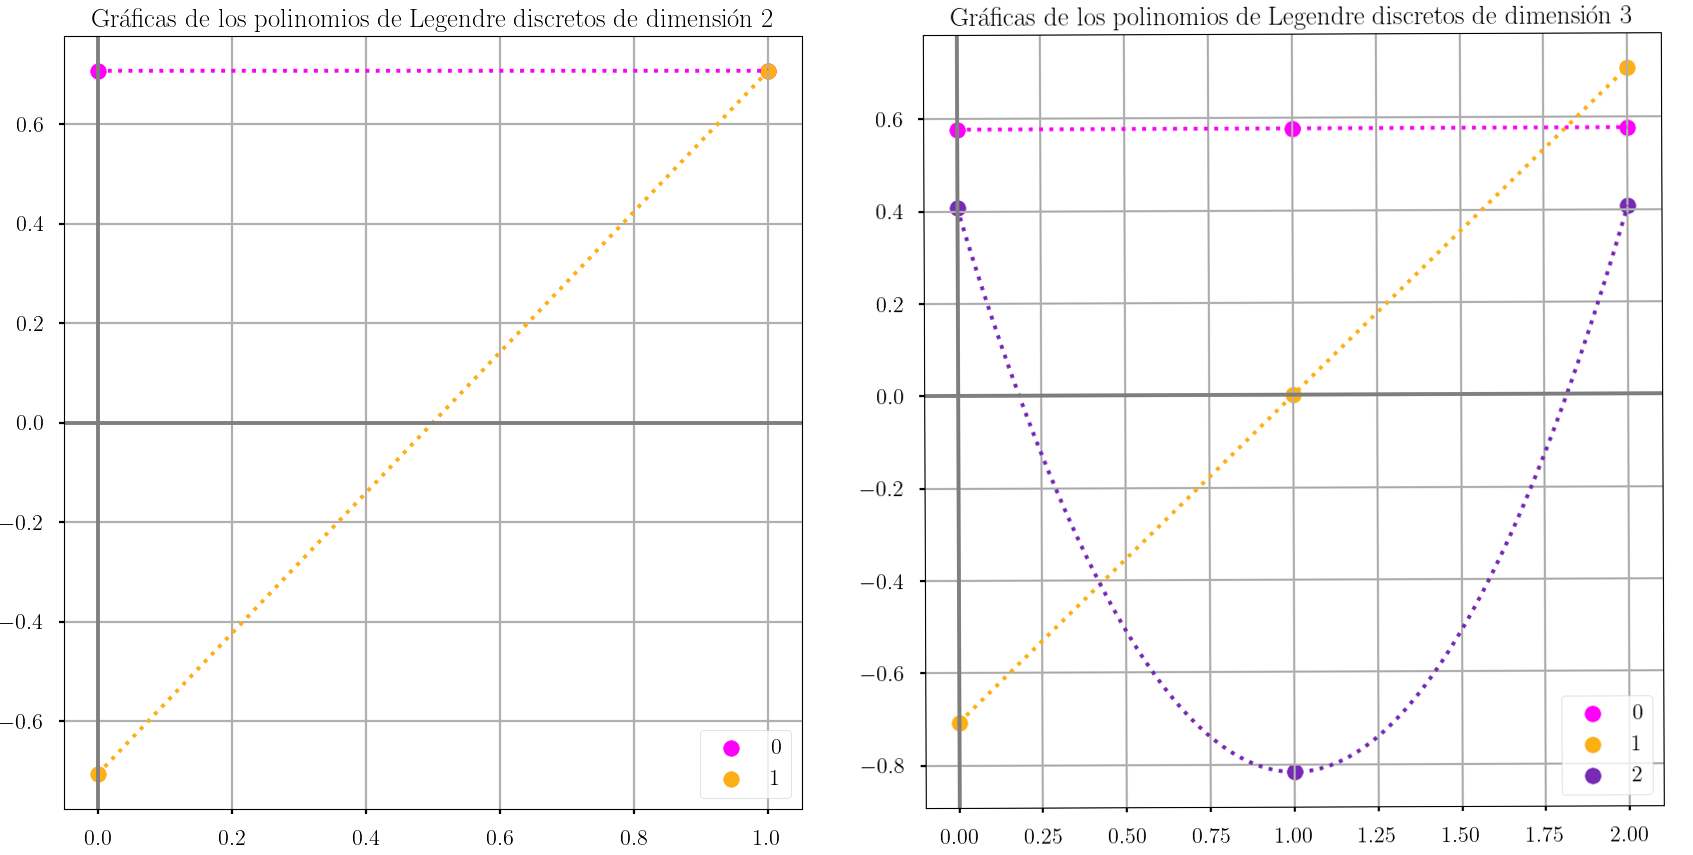
\includegraphics[scale = 0.9]{PDL_2_3} 
 \end{figure}	 
 \begin{figure}[H]
 	\sidecaption{
 	PDL de dimensiones $4$ y $5$.
 	\label{fig: PDL_dim2}
 	}
 	\centering
 	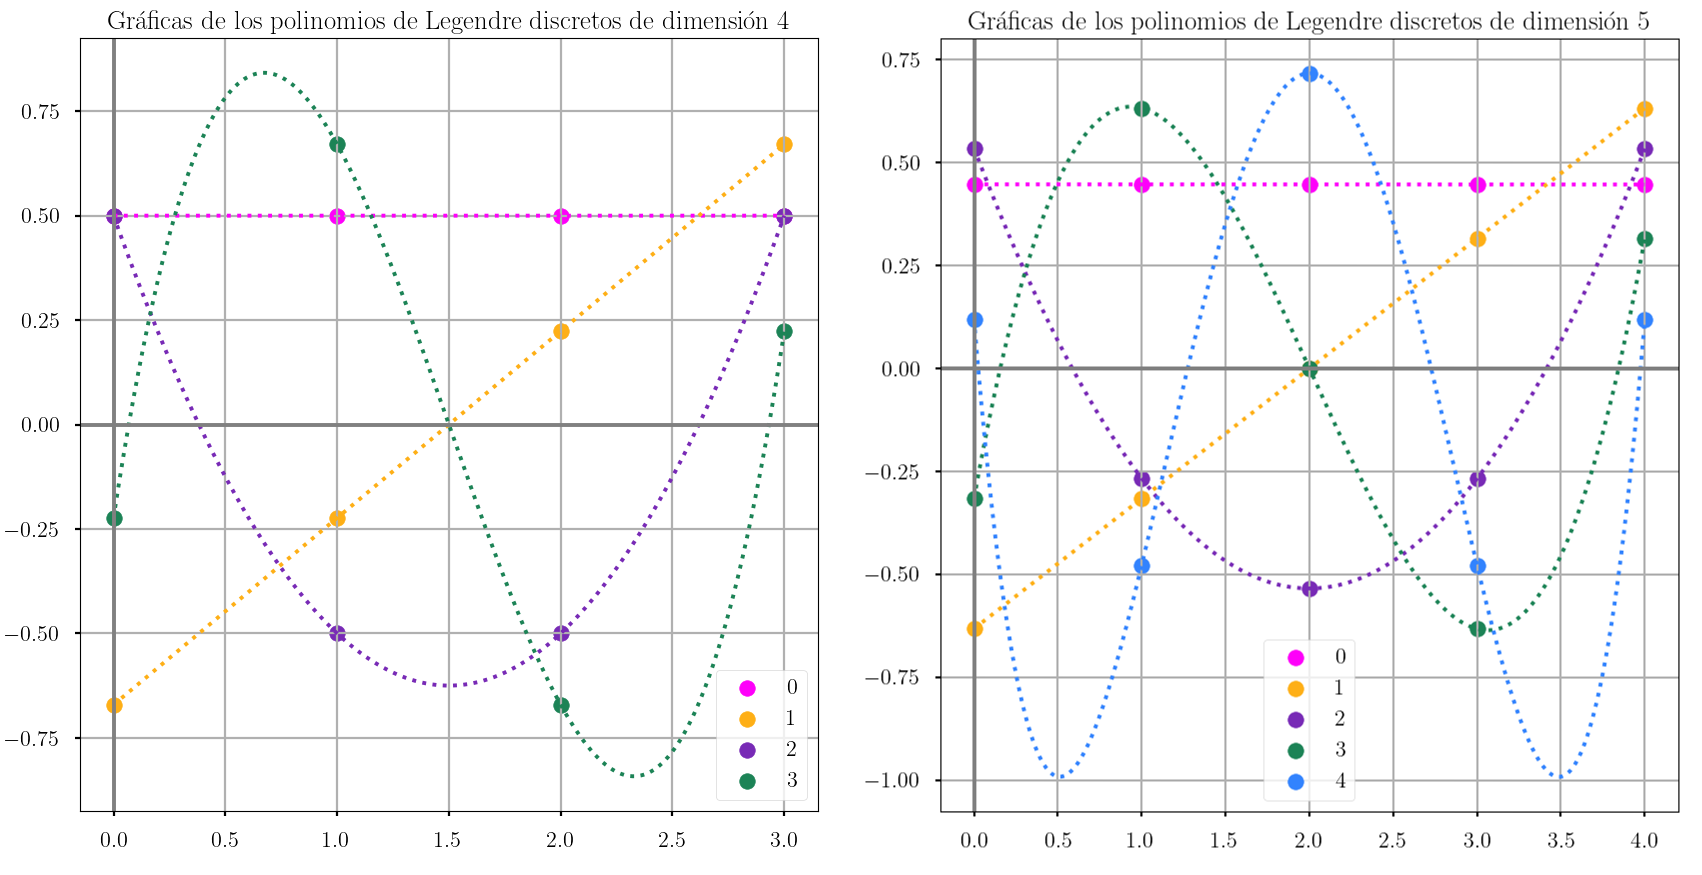
\includegraphics[scale = 0.9]{PDL_4_5} 
 \end{figure}	
 \begin{figure}[H]
 	\sidecaption{
 	PDL de dimensiones $6$ y $7$.
 	\label{fig: PDL_dim2}
 	}
 	\centering
 	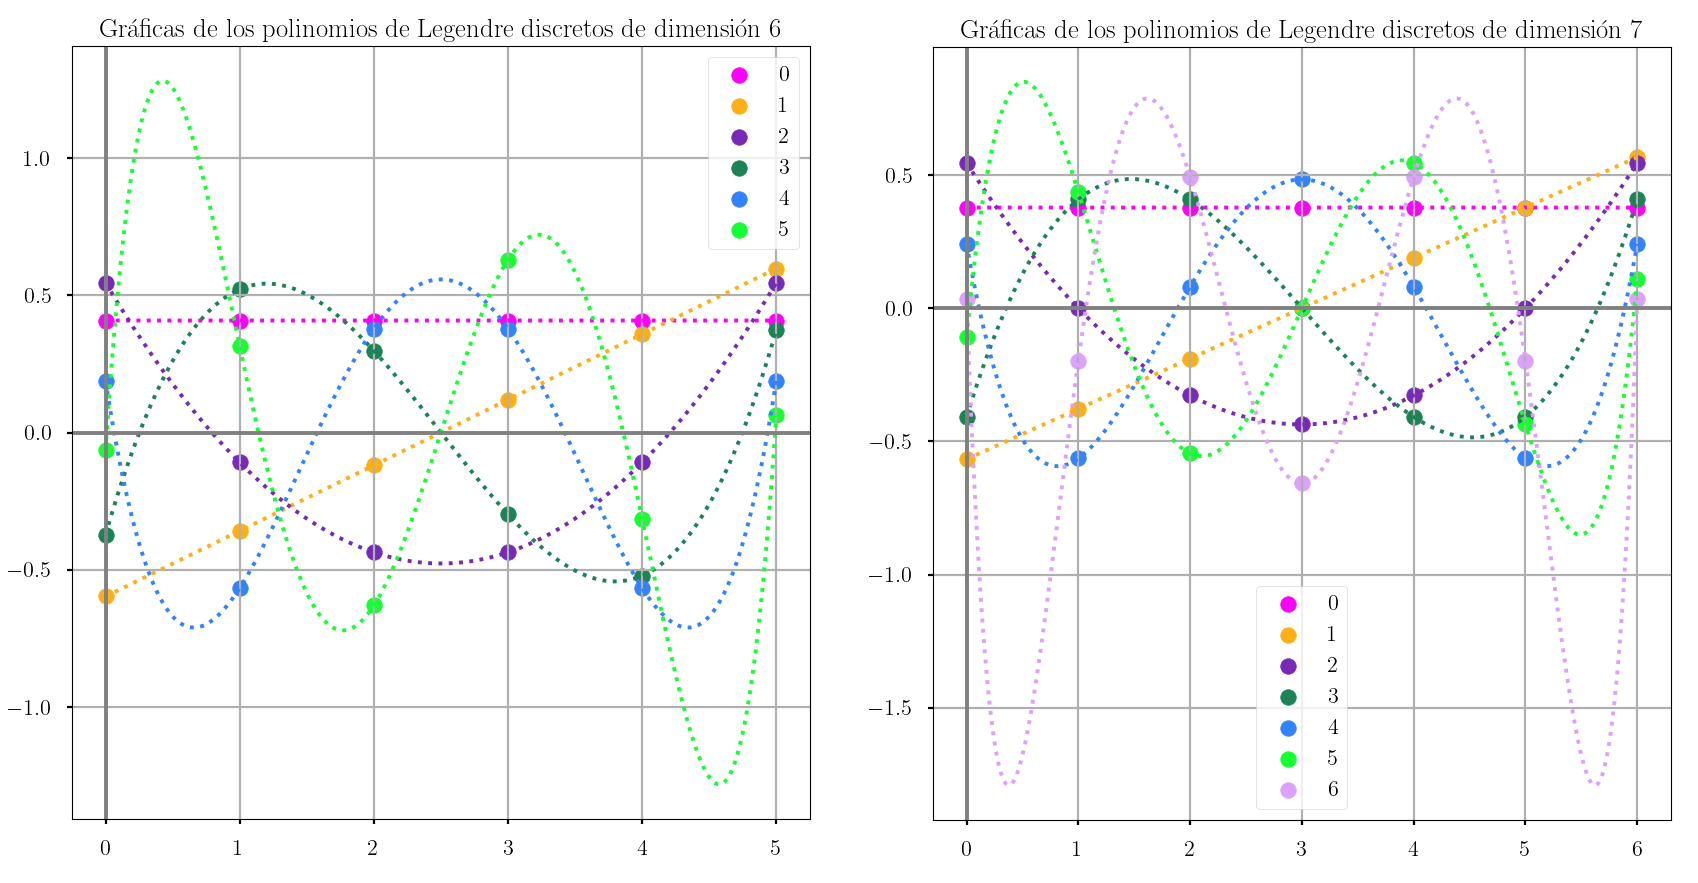
\includegraphics[scale = 0.9]{PDL_6_7} 
 \end{figure}	